\documentclass[sigconf]{acmart}
\setcopyright{none}

\AtBeginDocument{%
  \providecommand\BibTeX{{%
    Bib\TeX}}}

\settopmatter{printacmref=true}  % Ensures ACM reference format is included
\usepackage{balance}  % Load balance package for column balancing

\begin{document}

\title{Physics-Informed Neural Networks for Photoelectric-Compton Decomposition in Duel-Energy CT Tissue Classification}

\author{Karl Schmidt}
\email{karl.schmidt@colorado.edu}
\affiliation{%
  \institution{University of Colorado Boulder}
  \city{Boulder}
  \state{CO}
  \country{USA}
}

\acmConference[ ]{ }{ }{}
\acmBooktitle{}
\settopmatter{printacmref=false}
\renewcommand\footnotetextcopyrightpermission[1]{}

\begin{abstract}

Spectral computed tomography (Spectral CT) enables material-specific imaging by exploiting energy-dependent x-ray 
attenuation. However, accurate tissue decomposition—especially of low-prevalence classes like calcifications—remains 
challenging due to class imbalance, noise sensitivity, and limited ground truth data. This study introduces a
deep learning framework for tissue segmentation in dual-energy spectral CT. By leveraging the Beer–Lambert attenuation 
law and incorporating dual-energy attenuation maps \([\mu_{\text{low}}, \mu_{\text{high}}]\) as inputs, a U-Net-based 
convolutional neural networks (CNNs) is trained to segment adipose, fibroglandular, and calcified tissue. Two 
architectures, \texttt{UNet256} and \texttt{UNet512}, are evaluated, with the deeper \texttt{UNet512} model achieving 
superior performance (validation loss = 0.0292). Quantitative analysis shows close agreement between predicted and 
true tissue compositions, including for rare calcifications. This work demonstrates that using Beer–Lambert's law 
with Filtered Back Projection into CNN design enhances interpretability and segmentation accuracy, offering a reliable 
approach for tissue decomposition in spectral CT.

\vskip 2mm

  \textbf{Keywords:} Spectral CT, Clasification, Machine Learning, UNet, CNN

\end{abstract}


\maketitle

\section{Introduction}\label{sec:introduction}

Spectral Computed Tomography (Spectral CT) extends traditional CT by making use of the energy-dependence of
X-ray attenuation. The conventional CT process produces a single "grayscale" attenuation map which
can result in indistinguishable results when comparing similar bulk density materials. Spectral CT records
two separate x-ray photon energy spectra which allows for recording different attenuation properties
at different energies. Typically x-ray photons interact with materials through the photoelectric effect,
which typically occur at low photon energies, and Compton scattering, which typically occur at higher
photon energies. The dataset provided by the American Association of Physicists in Medicine (AAPM)
contains the "low-kVp" and "high-kVP" dual energy CT measurements collected at two different tube
voltages. The low-kVp transmission with the x-ray tube operating at 50 kVp and the high-kVp transmission 
operating at 80 kVp.

Extracting reliable photoelectric and Compton maps from noisy or limited‐view data is challenging. Classic
algebraic or statistical decomposition methods require careful regularization and often struggle with low
photon counts or beam‐hardening artifacts. Deep learning approaches, by contrast, can learn complex nonlinear
mappings but may overfit to the training distribution and produce physically inconsistent outputs (e.g.,
negative attenuation, or tissue maps that fail to reproduce the measured projection data).

This work proposes a basic Convolutional Neural Network (CNN) framework for multi‐energy CT tissue classification
where the output of the CNN will contain percentages of each tissue type - adipose, fibroglandular, and calcification.
By using the Beer-Lambert law, low- and high-kVp transmission data are converted into per‐pixel attenuation coefficients
before applying a closed-form basis decomposition to recover photoelectric and Compton component images. Effectively,
the low-energy region, 50 kVp, are considered the photoelectric effect interactions while the high-energy region, 80 kVp, 
are considered Compton scattering. 

These images are stacked and used with two core models with specific hyperparameter tuning to determine the model and
parameters which demonstrate the lowest Binary Cross Entropy (BCE) loss. The first model contains 11 convolutional layers 
structured in an encoder-decoder architecture. It downsamples the input images from 512×512 to a bottleneck of 128×128 
pixels, capturing mid-level semantic features before reconstructing the output at the original resolution. It's designed 
for moderately complex tasks with a balance between model depth and computational cost. The second model includes 15 
convolutional layers, adding an extra downsampling stage that allows the network to capture more abstract and global 
features. It also downsamples to a 128×128 latent space, despite having more layers, making it suitable for learning 
finer distinctions in more complex images or tasks.

The model is trained using the binary cross-entropy loss between the predicted tissue probability maps and the ground-truth i
phantom tissue labels. This loss directly penalizes voxel-wise deviations from the true tissue distribution.

During evaluation, the model’s output is also used to compute the mean tissue composition percentages across the image volume. 
These predicted percentages are compared to the true phantom percentages using an average absolute error metric, which provides 
an interpretable assessment of how well the model recovers the tissue mix — but this is not used for training.

This approach is applied on the publicly available AAPM DL-Spectral CT Challenge dataset \cite{AAPM2024SpectralCT},  performing comprehensive
EDA, sinogram-domain preprocessing, and network training entirely in PyTorch, with an explaination of future work that could
integrate ASTRA‐based differentiable forward projections.

\section{Related Work}\label{sec:related_work}

\section{Proposed Work}\label{sec:proposed_work}

\subsection{Problem Statement}\label{subsec:problem_Statement}

Accurate discrimination of soft‐tissue types in X‐ray computed tomography (CT) remains a
fundamental challenge in medical imaging. Conventional single‐energy CT produces grayscale
images in which different materials with similar attenuation coefficients (e.g.\,muscle 
vs.\,iodine‐enhanced blood or bone) can appear indistinguishable, leading to diagnostic 
ambiguity. Dual‐energy and photon‐counting CT systems acquire multiple energy‐resolved 
measurements, but extracting robust tissue‐specific maps from these spectral data is 
nontrivial: standard material‐decomposition methods are sensitive to noise, beam‐hardening, 
and detector imperfections, and purely data‐driven deep‐learning approaches often fail to 
generalize beyond their training domain.

This project proposes to address these limitations by developing a \emph{physics‐informed neural network} 
(PINN) that directly incorporates the known Beer–Lambert attenuation law and the two dominant 
interaction mechanisms—photoelectric absorption and Compton scattering—into its architecture 
and training loss. By decomposing each pixel’s dual‐energy attenuation pair \([\mu_{\rm low},\,
\mu_{\rm high}]\) into physically meaningful photoelectric and Compton components and enforcing 
consistency with both the measured attenuation maps and sinogram data, our approach aims to (1)
improve classification accuracy of key tissue types (adipose, fibroglandular, bone) and (2) 
enhance robustness to noise and out‐of‐distribution scenarios. This integration of first‐principles 
physics with modern deep learning promises more reliable, interpretable, and generalizable 
spectral CT tissue characterization.

\subsection{Data Preparation}\label{sec:data_preparation}

For building successful models, data mining is imperative to its success by ensuring data is collected,
clean, and preprocessed for use with each of the models before use. Data will be collected from various
locations and most likely in the form of comma separated value (CSV) data files. Given data will come
from different sources, it's time delta, size, shape, and time range were expected to be different. 
Data cleaning to concatenate these datasets into a single data source that includes features needed for
training and testing the model shall be performed. The cleaned dataset can then be stored in a parquet
columnar based file. 

Once the dataset is cleaned, a exploration of the data needs to be performed before using the dataset with
the models. This is where dataprocessing comes into affect. The exploratory data analysis (EDA) can be
informative for understanding the correlation between features in order to find potential multi-colinearity
issues within the data. This stage can also include adding data transformations to the final dataset. It is
understood within the blockchain community, that Bitcoin is a highly volatile asset. This volatility could
lead to overpredicting to the price noise. While some methods can be utilized to reduce overfitting, adding
a trailing average of previous price data can normalize direction of price movement.

\subsection{Price Prediction Methodology}\label{subsec:price_prediction_methodology}

Using AdaBoost, Random Forest, and Support Vector Machine models, a voting regressor will be used
to ensemble these models into a final price prediction. The general methodology for tuning these
individual models will be to utilize K-Fold and GridSearch to optimize a given set of parameters.

The implementation of these models will be done using the scikit-learn Python library.

\subsubsection{AdaBoost}\label{subsubsec:adaboost}

AdaBoost works by sequentially building models that correct the
errors made by previous models. Initially, a model is trained on the dataset, and subsequent models are built to address
the misclassifications of the prior models. This iterative process continues until errors are minimized, resulting in a
robust classifier. AdaBoost enhances prediction accuracy by combining multiple weak learners into a strong learner,
creating a powerful ensemble model. As an ensemble learning method, AdaBoost is particularly effective in improving the
performance of machine learning models by refining predictions through adaptive boosting\ \cite{adaBoostAnalyticsVidhya}.
From the scikit-learn library, the AdaBoostRegressor class will be used.

\subsubsection{Random Forest}\label{subsubsec:randomforest}

Random Forest is an ensemble learning technique that improves upon bagging by introducing a small but
crucial modification to decorrelate the decision trees. Like bagging, Random Forest constructs multiple
decision trees using bootstrapped training samples. However, when building each tree, the algorithm
randomly selects a subset of predictors (m) at each split, instead of considering all available
predictors (p). This random selection ensures that no single predictor dominates the splits, which
reduces the correlation between the trees. As a result, the predictions from the trees are more
independent, leading to a greater reduction in variance and more reliable results. In situations
with many correlated predictors, using a smaller subset of predictors (m) at each split helps improve
model performance by preventing overfitting and increasing the diversity of the trees. This technique
has been particularly effective in high-dimensional data, such as predicting cancer types based on
gene expression data, where the model shows improved prediction accuracy over bagging\ \cite{James2023}.
RandomForestRegressor will be used. 

\subsubsection{Support Vector Machine}\label{subsubsec:svm}

The support vector machine (SVM) is an advanced version of the maximal margin classifier, a simple and
intuitive binary classifier that aims to separate two classes using a linear boundary. However, the
maximal margin classifier is not suitable for most real-world datasets, as it requires the classes to be
perfectly separable by a linear boundary. To address this limitation, the support vector classifier (SVC)
was introduced as an extension, allowing for some flexibility by permitting misclassifications to improve
robustness and generalizability. The support vector machine further extends the SVC by handling non-linear
class boundaries, making it applicable to a wider range of datasets. Additionally, SVMs can be adapted for
multi-class classification, and they share strong connections with other statistical methods like logistic
regression, providing a powerful framework for binary and multi-class classification tasks\ \cite{James2023}.
For the SVM implementation, the  SVR class will be used with a radial base function kernel. 

\subsubsection{Voting Regressor}\label{subsubsec:voting_regressor}

A Voting Regressor is an ensemble learning technique that combines predictions from multiple regression models to improve
the accuracy and robustness of predictions. It aggregates the outputs of various base models, typically through averaging,
to create a stronger final prediction. This helps in reducing the risk of overfitting compared to relying on a single model.
The Voting Regressor can accommodate different types of regressors (such as Linear Regression, Random Forest, and Support
Vector Regression) and allows for weighted combinations of their predictions. By assigning different weights to each model
based on its performance, the Voting Regressor can further enhance prediction accuracy. This ensemble method is effective
in improving the generalization of machine learning models by leveraging the strengths of multiple base
regressors\ \cite{votingRegressorMedium}.

\section{Evaluation}\label{sec:evaluation}

Utilizing a 80/15/15 training, test, and validation set, each model will be tuned by mean squared error (MSE) which helps
interpret how our model performance from a variance perspective, mean absolute error (MAE) for evaluating precision, and
the Coefficient of Determination (R2) to help understand how well the models outcomes describe the feature set. Cross
Validation will also be used to show how well each individual model is performing. This could be a good indicator as 
each model will be tuned with scikit-learn's KFold cross-validation class with 5 folds each. In addition, each model will
be given a set of hyperparameter values that will be run through the GridSearchCV for selecting the best combination.
The best hyperparameters will then be evaluated based on MSE, MAE, and R2. 

\subsection{Data Preparation}\label{sec:data_preparation_eval}

\subsection{Data Collection}\label{sec:data_collection}

Data was collected from multiple sources: the U.S. Dollar Index (DXY), Bitcoin data, and the M2 Money Supply (M2SL). Each
dataset is retrieved from CSV files located in the data directory, and the date range for the data collection is restricted
between \textbf{January 1, 2017} and \textbf{September 2, 2023}.

\subsubsection{Bitcoin Data}\label{sec:bitcoin_data}

Harris' Bitcoin network dataset\ \cite{bitcoinData} is a Kaggle dataset that contains several CSV files pertaining to Bitcoin on-chain, network, and
price data. This project only uses the daily Bitcoin daily data which includes calculated values such as the
Fear and Greed index, dervied from metrics within the Bitcoin network.

\begin{itemize}
    \item \textbf{Granularity:} Daily (from 2009 to 2023)
    \item \textbf{Size:} 12 columns, 666 rows
    \item \textbf{Data Columns:}
    \begin{itemize}
        \item datetime
        \item \textbf{market\_price\_usd}: The Bitcoin price in USD
        \item \textbf{total\_supply}: The total supply of Bitcoin tokens
        \item \textbf{market\_cap\_usd}: The total market capitalization of Bitcoin in USD
        \item \textbf{realised\_cap\_usd}: The value of the Bitcoin network based on the price at which each coin last moved on-chain
        \item \textbf{nupl}: Net Unrealized Profit/Loss, calculated as the market capitalization minus realized capitalization, divided by market capitalization
        \item \textbf{coin\_days\_destroyed}: A measure of the number of coins transacted and how long they remained unspent
        \item \textbf{active\_addresses}: The number of daily active Bitcoin addresses
        \item \textbf{fear\_greed\_value}: A sentiment indicator measuring market emotions, ranging from extreme fear (0\-24) to extreme greed (75\-100)
        \item \textbf{fear\_greed\_category}: The category of the Fear and Greed Index
        \item \textbf{lightning\_nodes}: The number of nodes running on the Lightning Network
        \item \textbf{lightening\_capacity\_usd}: The total value of Bitcoin (in USD) locked in the Lightening Network
    \end{itemize}
\end{itemize}

\subsubsection{M2 Money Supply}\label{sec:m2_money_supply}

The M2 Money Supply (M2S) is a broad measure of the total amount of dollars circulating in the economy. The Fred
\ \cite{m2slData} dataset is
included because the supply of money is often correlated with the appreciation of various assets, including Bitcoin,
within macroeconomic trends. Typically, Bitcoin's price experiences high and low peaks around a four-year cycle, which
may correlate with M2S, especially considering the effects of quantitative easing (QE) and quantitative tightening (QT)
implemented by the Federal Reserve. QE generally occurs when the U.S. government extends the debt limit, often in
response to the need to pay off national debt, which leads to inflation. The Federal Reserve typically responds to this
inflation by removing money from circulation.

\begin{itemize}
    \item \textbf{Granularity:} Monthly (from 1960 to 2025)
    \item \textbf{Size:} 2 columns, 770 rows
    \item \textbf{Data Columns:}
    \begin{itemize}
        \item \textbf{observation\_date}: The month for each M2S data reading
        \item \textbf{M2SL}: The total money supply.
    \end{itemize}
\end{itemize}

\subsubsection{ISM Manufacturing PMI}\label{ism_manufacturing_pmi}

The ISM Manufacturing PMI (Purchasing Managers' Index) is a key economic indicator that measures the economic health of
the manufacturing sector in a country, specifically the United States. It is released monthly by the Institute for Supply
Management (ISM). The U.S. Dollary Index (DXY) dataset\ \cite{dxyData} contains daily index value data.

\begin{itemize}
    \item \textbf{Granularity:} Daily (from 2014 to 2023)
    \item \textbf{Size:} 4 columns, 2502 rows
    \item \textbf{Data Columns:}
    \begin{itemize}
        \item \textbf{open}: The daily opening index value
        \item \textbf{high}: The daily high index value
        \item \textbf{low}: The daily low index value
        \item \textbf{close}: The daily close index value
    \end{itemize}
\end{itemize}

\subsubsection{Data Cleaning}\label{sec:data_cleaning}

The data collection and preprocessing workflow involves multiple steps to ensure that the datasets are correctly
formatted, synchronized, and cleaned before further analysis. The following steps summarize the data cleaning process:

Each dataset includes a date column, which is converted to a \texttt{datetime} format using \texttt{pandas.to\_datetime()}.
This ensures uniformity in the way dates are represented across the datasets. The specific format for each dataset was
handled (e.g., MM/DD/YYYY format for the DXY data), and any invalid or malformed date entries were coerced to \texttt{NaT}
(Not a Time).

After parsing the dates, each dataset was filtered to ensure that only data within the specified date range (from
\textbf{January 1, 2017} to \textbf{September 2, 2023}) is retained. This ensures that the analysis is consistent and
relevant to the chosen time period.

The date column names were standardized across all datasets. The \texttt{Date} column in the DXY dataset was renamed to
\texttt{date}, and similarly, the \texttt{datetime} column in the Bitcoin dataset and the \texttt{observation\_date}
column in the M2SL dataset were renamed to \texttt{date} to facilitate merging and avoid potential issues with inconsistent
column names.

The next step involved merging the individual datasets into a single dataframe. A date range dataframe was created to
ensure that the data spans the full range of dates from \textbf{January 1, 2021} to \textbf{September 2, 2023}. This date
range was used as a reference to merge all three datasets (DXY, Bitcoin, and M2SL) on the common \texttt{date} column.
The merging strategy used was a \textbf{left join}, ensuring that no dates were missed in the final dataset.

After the merge, the datasets were forward-filled to replace any missing values with the last valid entry, using
\texttt{ffill()}. This is particularly useful in time-series data where missing values are often caused by non-reporting on
certain days. Subsequently, any remaining rows with missing values were removed using \texttt{dropna()}, ensuring the final
dataset does not contain incomplete rows.

The result of the merging and cleaning process is a single, consolidated dataframe with synchronized, cleaned data from
the DXY, Bitcoin, and M2SL datasets, ready for further analysis. The data is now aligned by date, with missing entries
appropriately handled and all columns renamed consistently.

The cleaned data is now ready for subsequent analysis, ensuring the integrity of the datasets and their alignment across
all data sources.

\subsection{Exploratory Data Analysis}\label{sec:exploratory_data_analysis}

In this section, we provide a summary of the key statistics for several important features related to the market data,
realised capitalization, network metrics, and macroeconomic factors. The tables below present the descriptive
statistics for each feature, such as the count, mean, standard deviation, and percentiles.

Table\ \ref{tab:market_data} shows the summary statistics for the market data, including the market price, total supply,
and market capitalization. The data spans across 2040 observations.

Table\ \ref{tab:market_data_cont} continues with additional metrics related to the market,
such as the realised capitalization, NUPL (Net Unrealized Profit and Loss), and coin days destroyed.

Table\ \ref{tab:lightning_network} provides an overview of the lightning network statistics,
including the number of lightning nodes and their corresponding capacity.

Finally, Table\ \ref{tab:on_chain_metrics} presents summary statistics for the on-chain metrics and
macroeconomic variables, including active addresses, fear \& greed index, DXY, and M2SL.\

\begin{table}[ht]
    \centering
    \begin{tabular}{|l|c|c|c|c|}
    \hline
    Statistic & date    & Market Price & Total Supply & Market Cap. \\ \hline
    count     & 2040.00 & 2040.00      & 2040.00      & 2040.00     \\ \hline
    mean      & .2f     & 21179.31     & 18388710.96  & 396949466128.52 \\ \hline
    min       & .2f     & 3236.72      & 16839677.00  & 56399873657.69  \\ \hline
    25\%      & .2f     & 8115.03      & 17782030.25  & 142190217496.98 \\ \hline
    50\%      & .2f     & 16210.51     & 18545873.50  & 304886044680.10 \\ \hline
    75\%      & .2f     & 30464.50     & 19008497.00  & 589148933349.78 \\ \hline
    max       & .2f     & 67492.00     & 19473739.00  & 1273420650592.18 \\ \hline
    std       & nan     & 16228.93     & 745281.68    & 309020614744.35 \\ \hline
    \end{tabular}
    \caption{Summary Statistics: Market Data}
    \label{tab:market_data}
\end{table}

\begin{table}[ht]
    \centering
    \begin{tabular}{|l|c|c|c|}
    \hline
    Statistic & Realised Cap    & NUPL    & Coin Days Destroyed \\ \hline
    count     & 2040.00         & 2040.00 & 2040.00             \\ \hline
    mean      & 239097911053.34 & 0.30    & 10637974.16         \\ \hline
    min       & 76222559953.09  & -0.43   & 1313012.07          \\ \hline
    25\%      & 91240764924.07  & 0.20    & 4581202.29          \\ \hline
    50\%      & 129846243343.62 & 0.35    & 6724452.11          \\ \hline
    75\%      & 392646325879.52 & 0.46    & 11456585.84         \\ \hline
    max       & 468557597880.42 & 0.75    & 397370509.67        \\ \hline
    std       & 153945860647.49 & 0.25    & 16222122.31         \\ \hline
    \end{tabular}
    \caption{Summary Statistics: Market Data continued}
    \label{tab:market_data_cont}
\end{table}

\begin{table}[ht]
    \centering
    \begin{tabular}{|l|c|c|}
    \hline
    Statistic & Lightening Nodes & Lightening Capacity \\ \hline
    count     & 2040.00          & 2040.00             \\ \hline
    mean      & 9904.04          & 57127638.51         \\ \hline
    min       & 0.00             & 0.00                \\ \hline
    25\%      & 4569.00          & 6193676.69          \\ \hline
    50\%      & 7716.00          & 16873160.32         \\ \hline
    75\%      & 17087.00         & 111777070.67        \\ \hline
    max       & 20707.00         & 216470149.70        \\ \hline
    std       & 6541.46          & 60498632.08         \\ \hline
    \end{tabular}
    \caption{Summary Statistics: Lightning Network}
    \label{tab:lightning_network}
\end{table}

\begin{table}[ht]
    \centering
    \begin{tabular}{|l|c|c|c|c|}
    \hline
    Statistic & Active Addresses & Fear \& Greed & DXY     & M2SL     \\ \hline
    count     & 2040.00          & 2040.00       & 2040.00 & 2040.00  \\ \hline
    mean      & 857633.10        & 43.21         & 97.49   & 18178.32 \\ \hline
    min       & 410502.00        & 5.00          & 88.59   & 13907.30 \\ \hline
    25\%      & 728823.00        & 25.00         & 93.58   & 14782.90 \\ \hline
    50\%      & 874279.00        & 40.00         & 96.90   & 18972.90 \\ \hline
    75\%      & 974841.00        & 57.00         & 100.48  & 21117.10 \\ \hline
    max       & 1368431.00       & 95.00         & 114.10  & 21723.20 \\ \hline
    std       & 169318.22        & 21.53         & 5.17    & 3005.79  \\ \hline
    \end{tabular}
    \caption{Summary Statistics: On-chain Metrics and Macro}
    \label{tab:on_chain_metrics}
\end{table}

\begin{figure}[h]
    \centering
    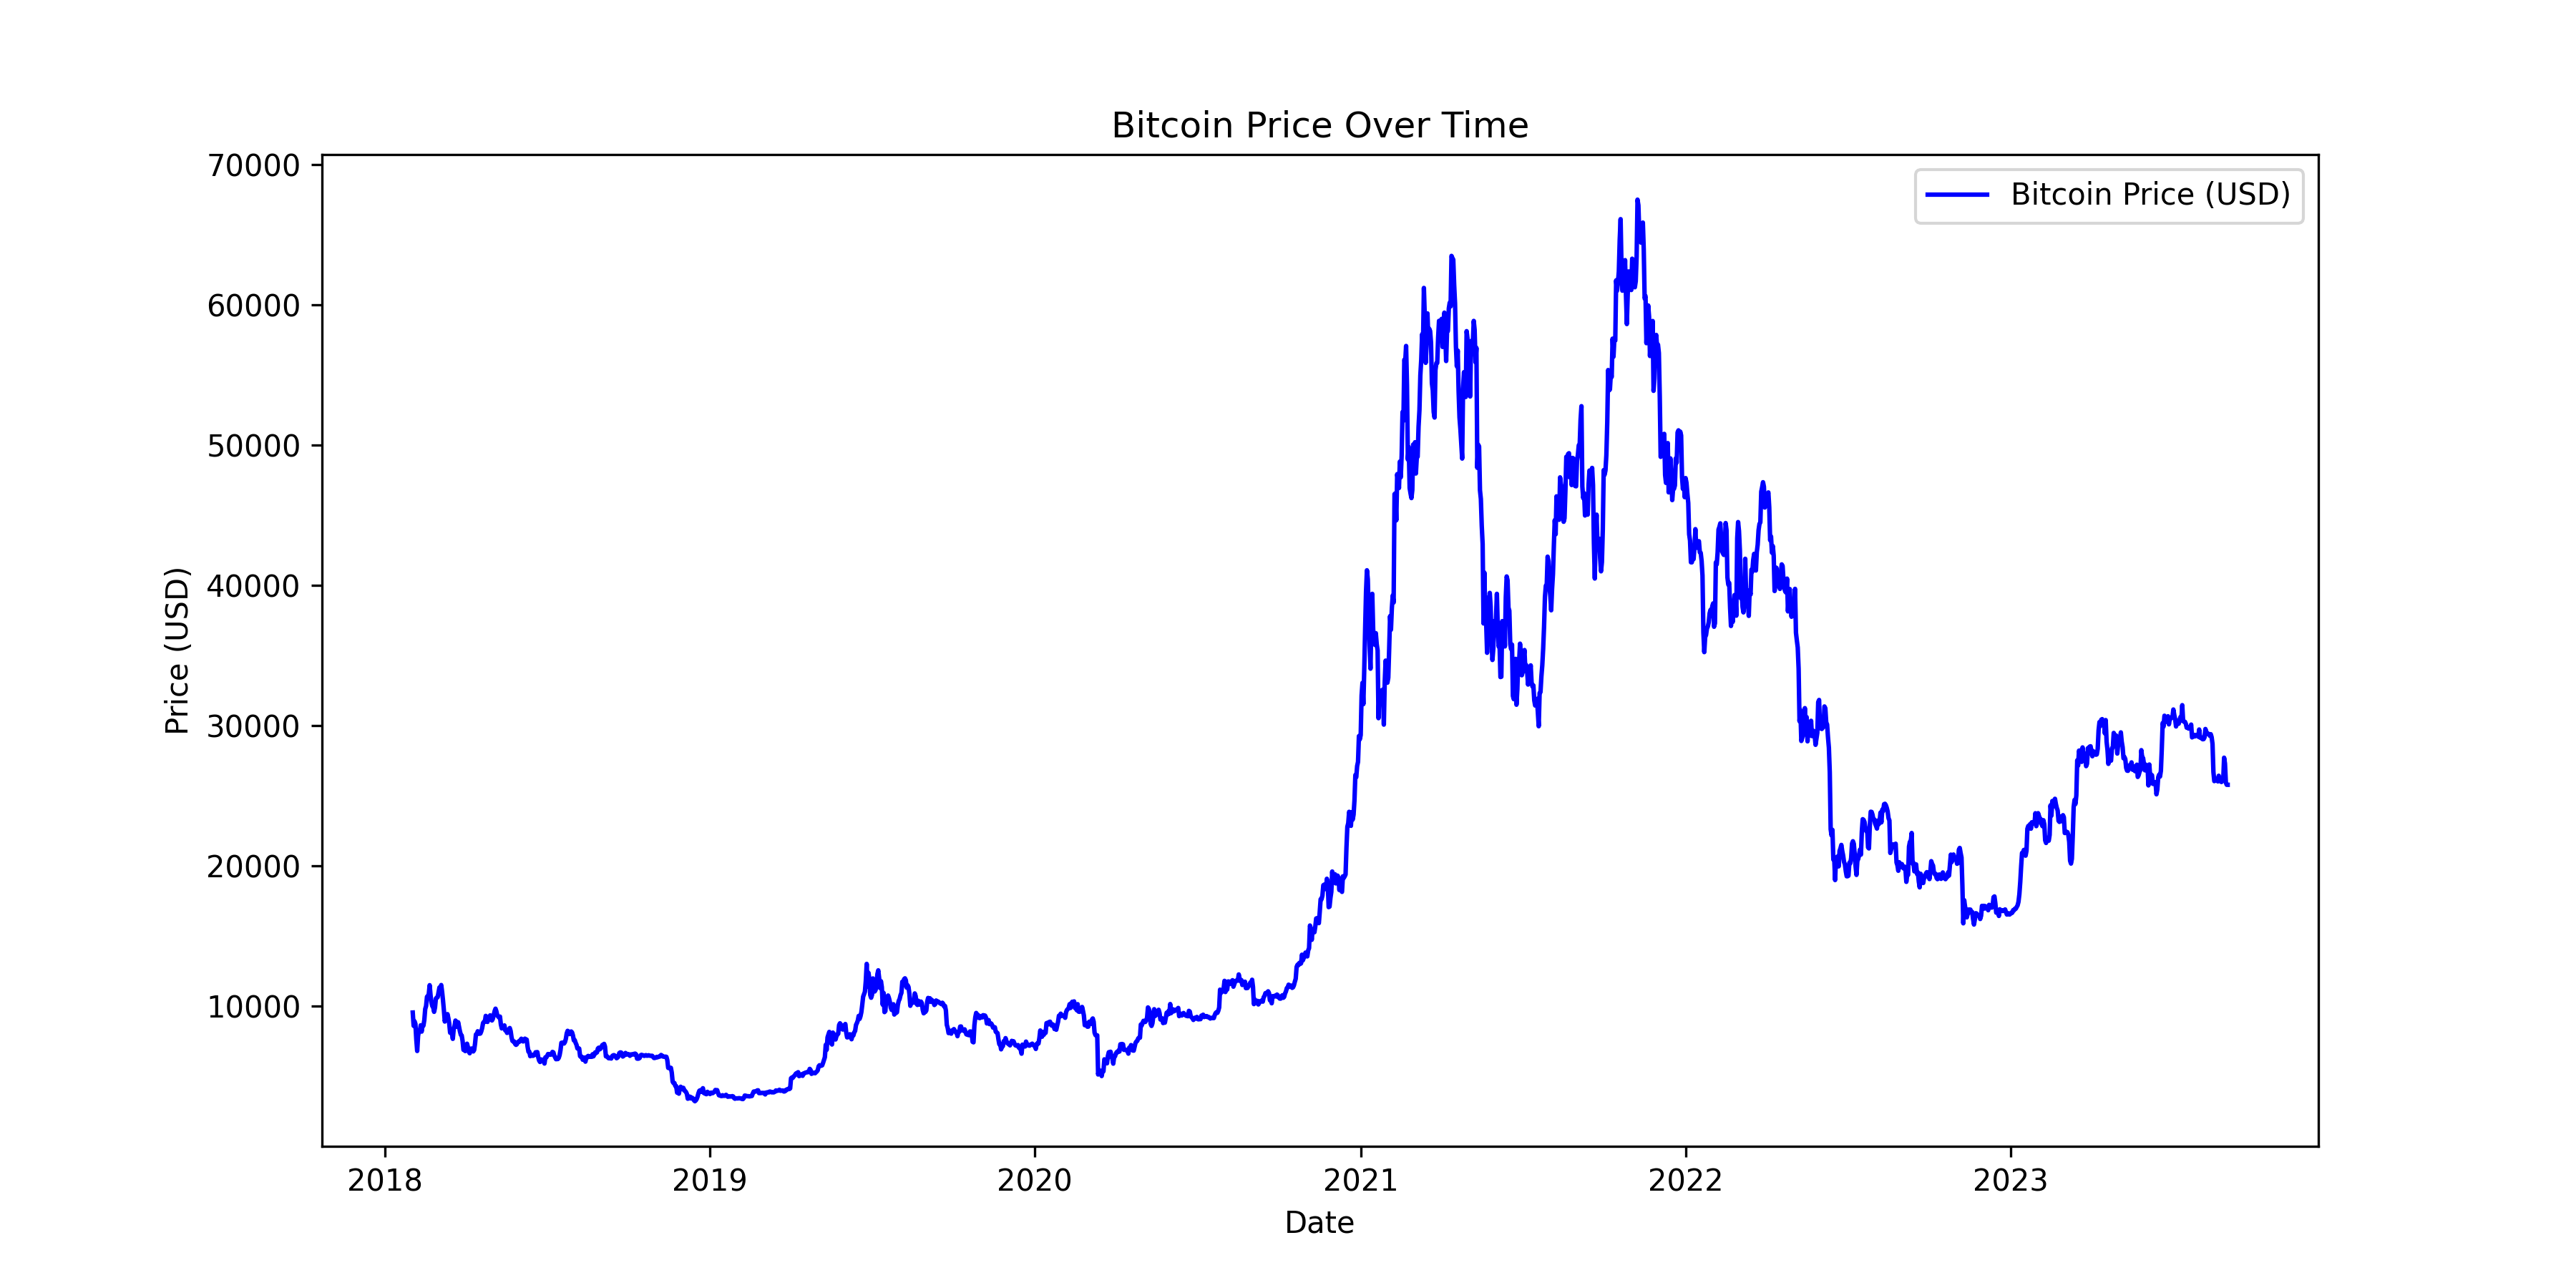
\includegraphics[width=0.5\textwidth]{plots/bitcoin_price_plot.png} % Replace with your file path
    \caption{Bitcoin Price Data.}
    \label{fig:bitcoin_price}
\end{figure}

Figure \ref{fig:example_plot} displays the price data of Bitcoin over time. This figure illustrates the fluctuations
in Bitcoin's market price, which reflects the volatility characteristic of cryptocurrency markets. From this plot,
we can observe periods of significant growth, as well as sharp declines, which are typical of the high-risk,
high-reward nature of digital asset trading.


\begin{figure}[h]
    \centering
    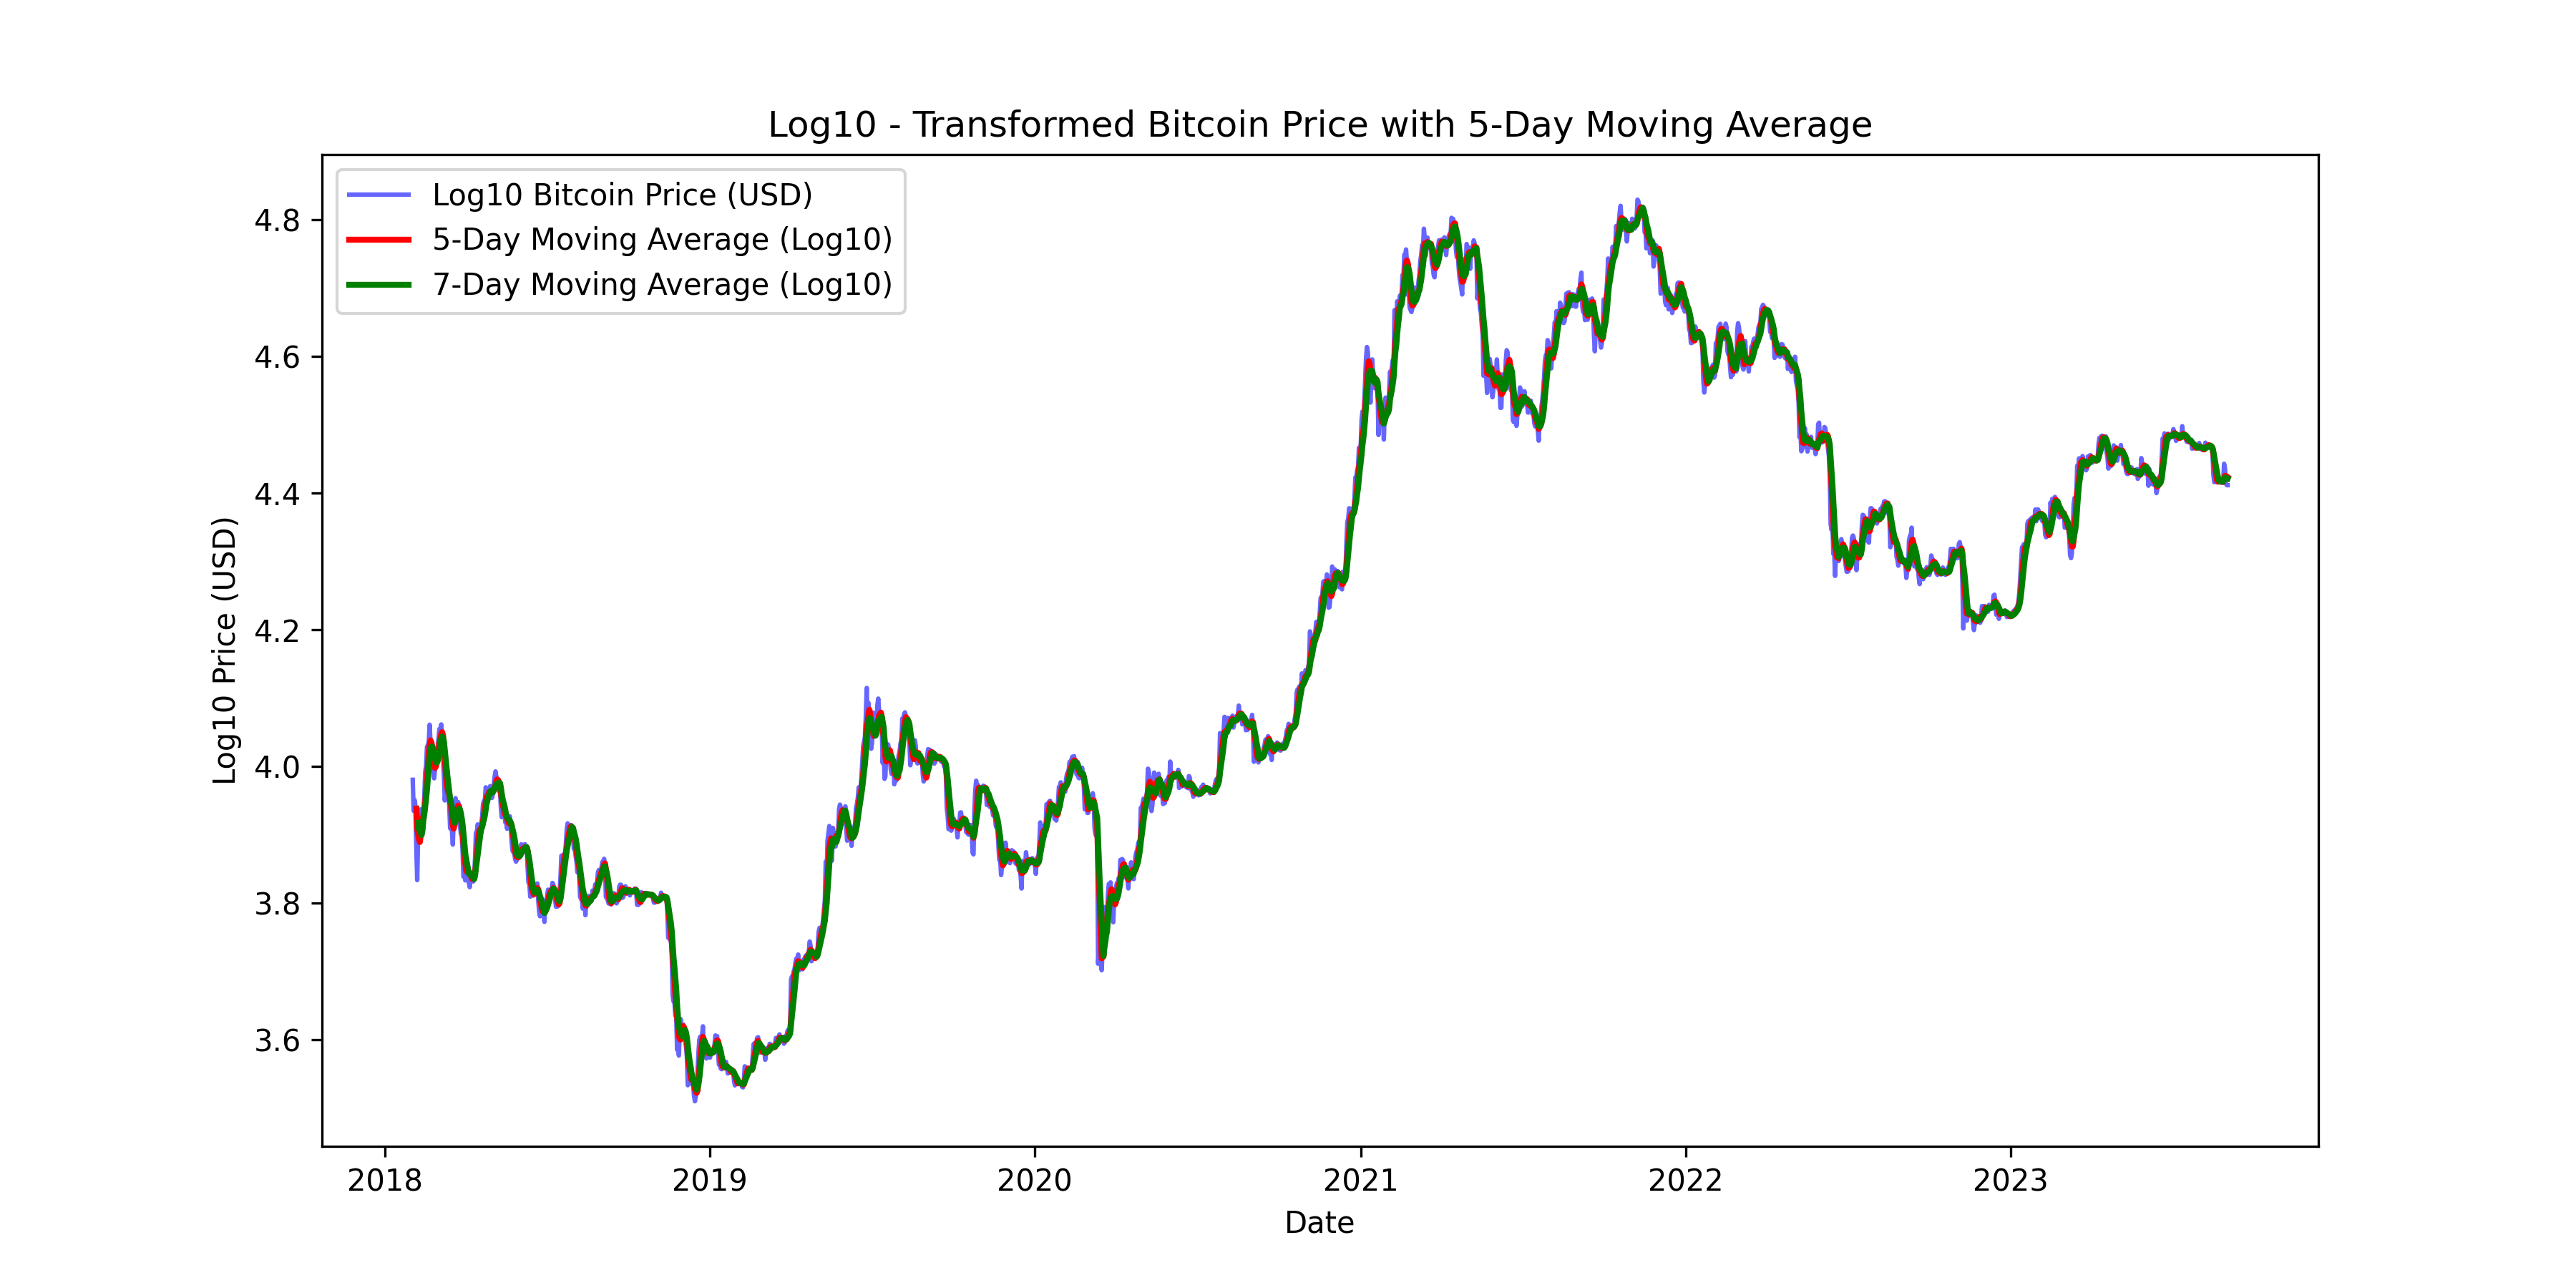
\includegraphics[width=0.5\textwidth]{plots/trailing_average_plot.png} % Replace with your file path
    \caption{Price Trailing Average.}
    \label{fig:trailing_average}
\end{figure}

Figure\ \ref{fig:trailing_average} presents the trailing average of Bitcoin's price, which smooths out short-term
fluctuations to provide a clearer picture of the overall trend. By calculating the average over a specified time
window, the figure helps in understanding the general direction of Bitcoin’s market price, indicating potential
periods of stability or volatility. This figure is crucial for analyzing market sentiment and trends.


\begin{figure}[h]
    \centering
    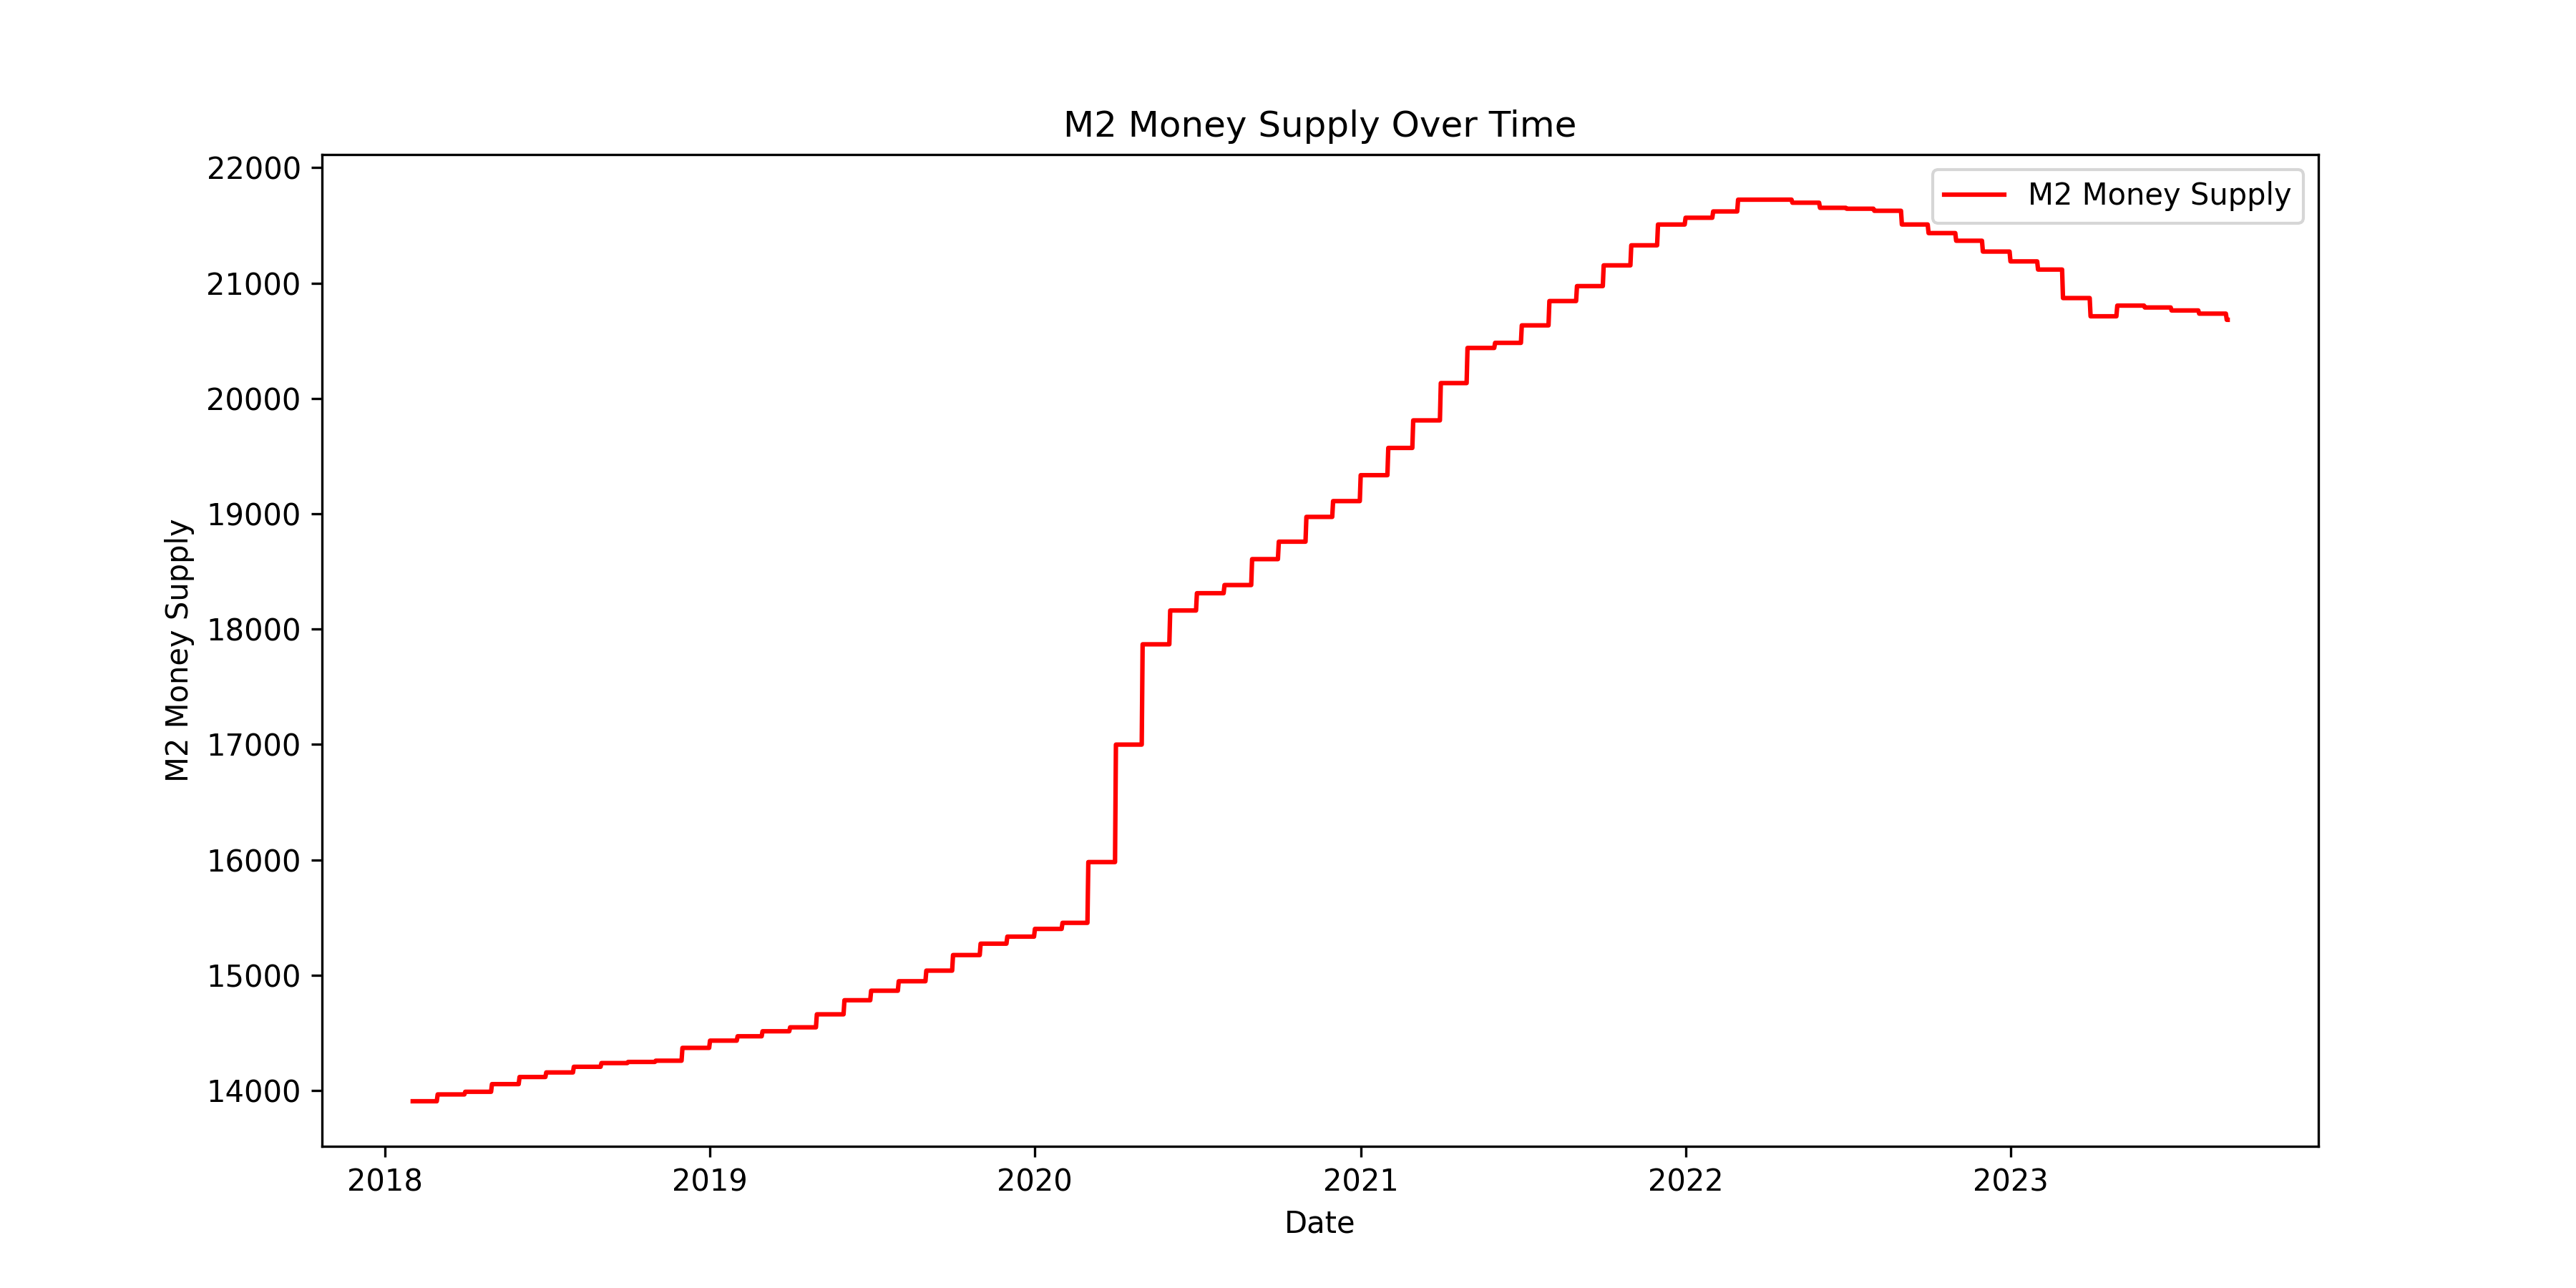
\includegraphics[width=0.5\textwidth]{plots/m2sl_plot.png} % Replace with your file path
    \caption{M2 Money Supply.}
    \label{fig:m2sl}
\end{figure}

Figure\ \ref{fig:m2sl} depicts the M2 Money Supply (M2SL) over time, showing the total supply of money in the
economy, including currency, checking, and savings accounts, and other near money assets. The M2SL data is often
used as a macroeconomic indicator to assess inflationary pressure or potential economic growth. This figure provides
context on how changes in money supply correlate with the Bitcoin market, especially during times of economic uncertainty.


\begin{figure}[h]
    \centering
    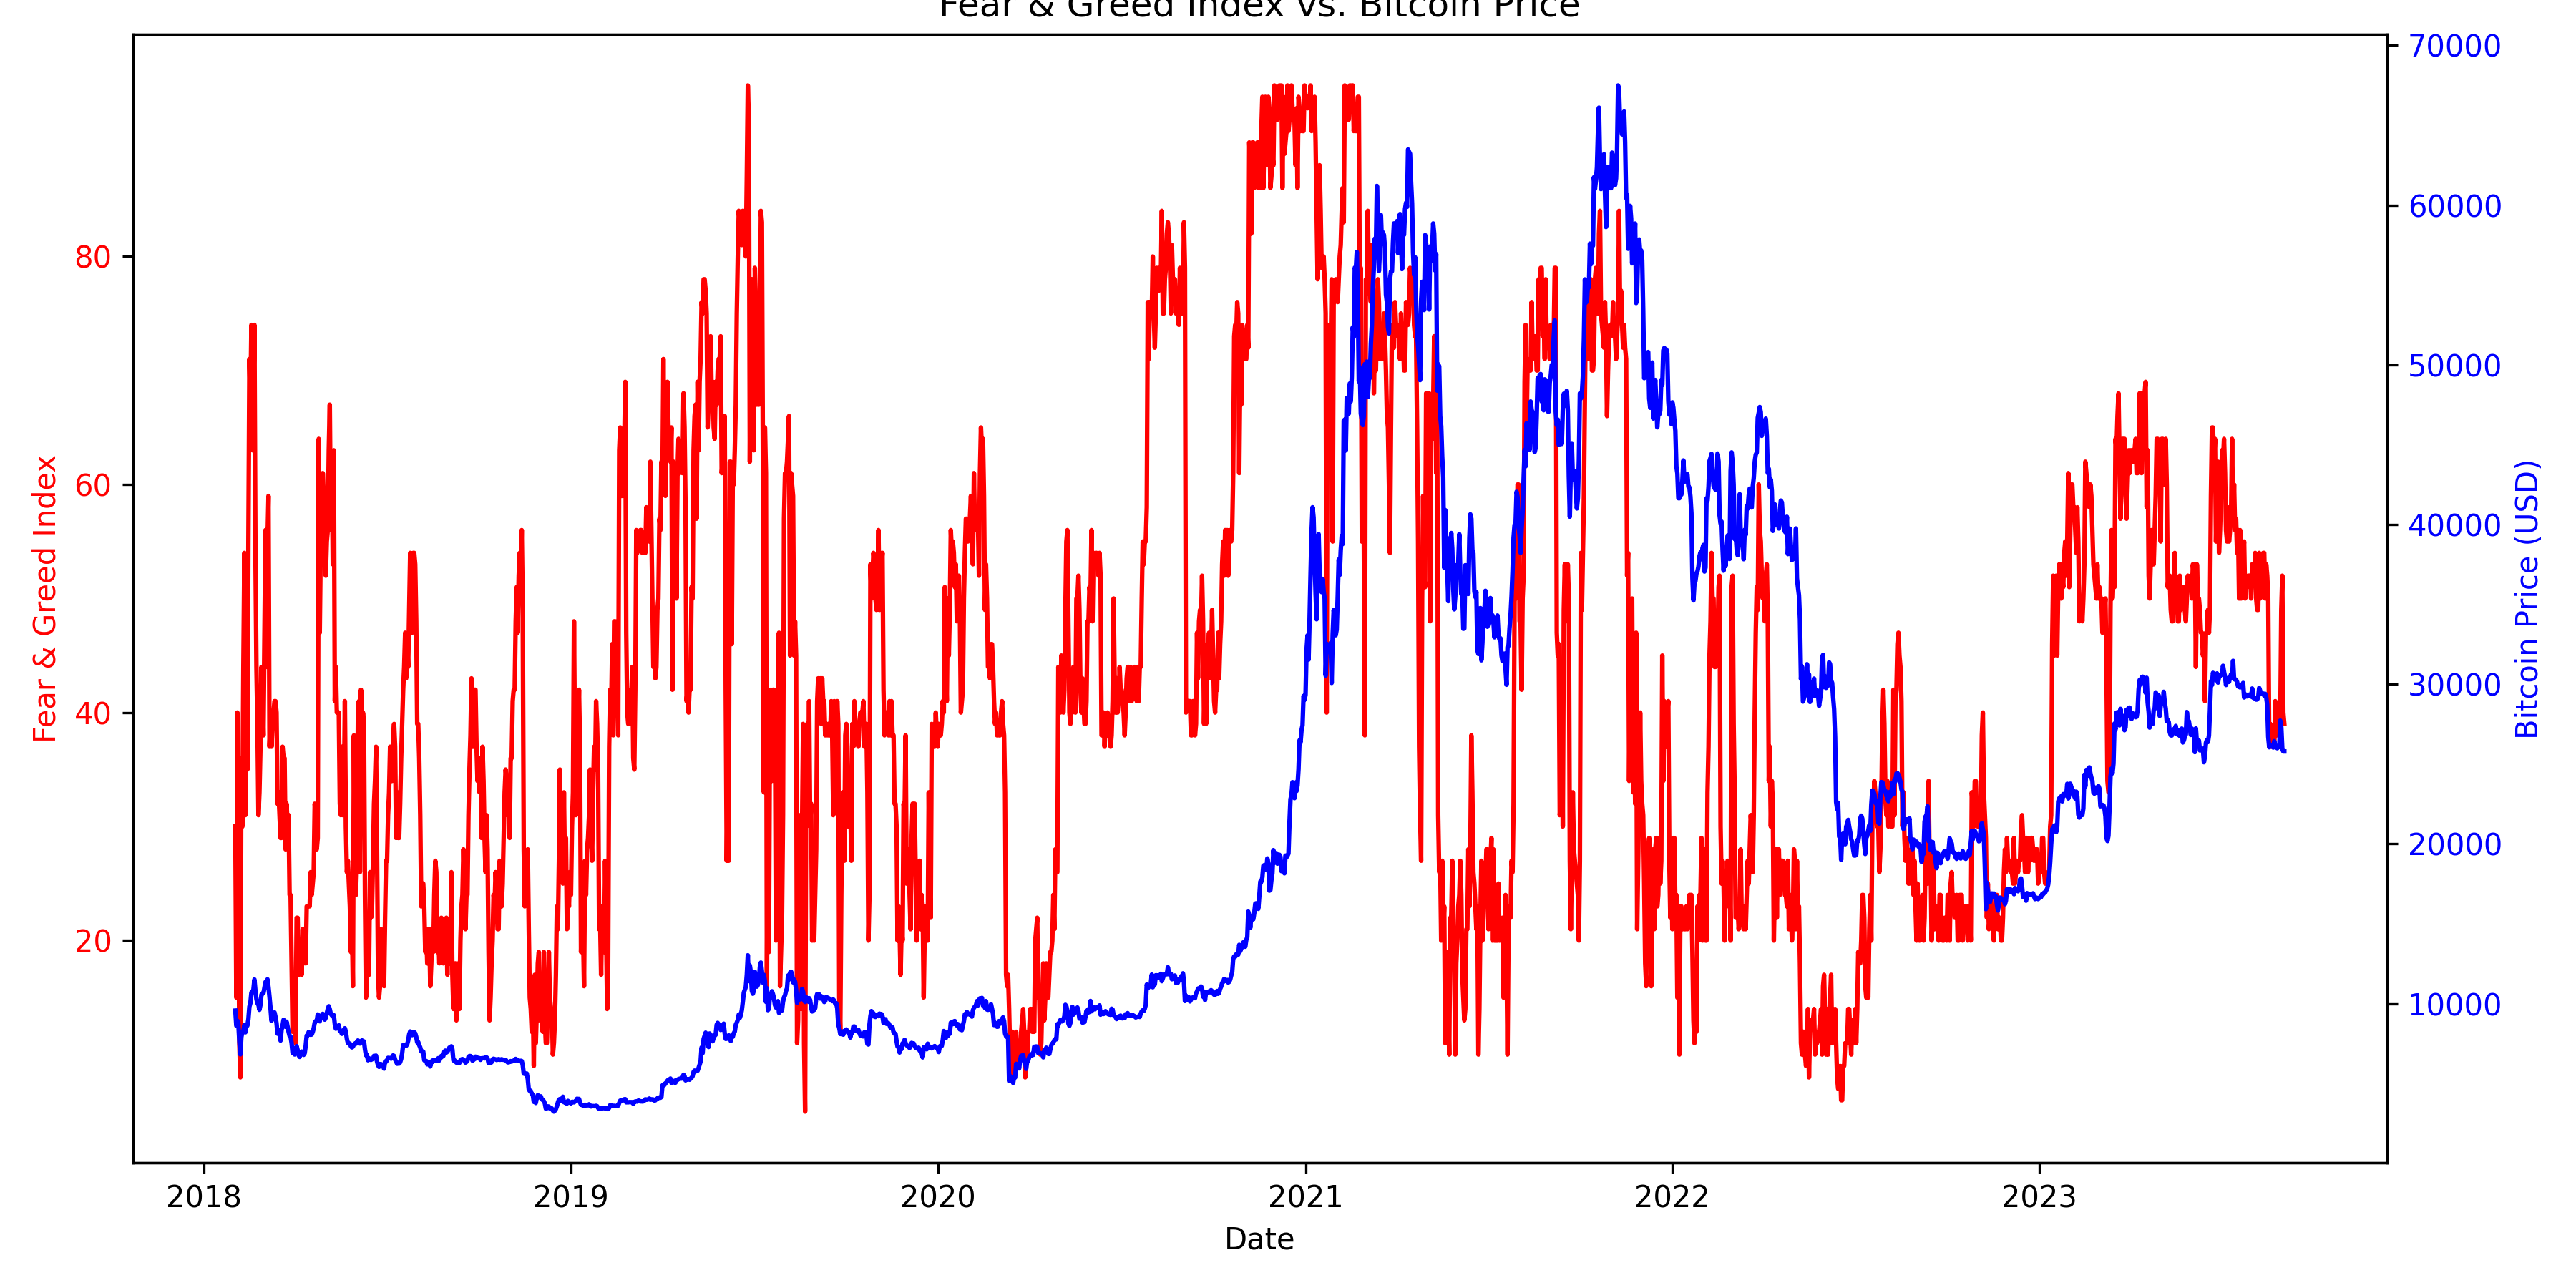
\includegraphics[width=0.5\textwidth]{plots/fear_and_greed_plot.png} % Replace with your file path
    \caption{Fear and Greed.}
    \label{fig:fear_and_greed}
\end{figure}

Figure\ \ref{fig:fear_and_greed} illustrates the Fear and Greed index, which measures the sentiment of investors in
the market. The index ranges from extreme fear to extreme greed, offering insights into how market participants feel
about Bitcoin's future prospects. Understanding this sentiment can aid in predicting potential price movements, as
extreme levels of fear or greed often signal market corrections or bubbles.


\begin{figure}[h]
    \centering
    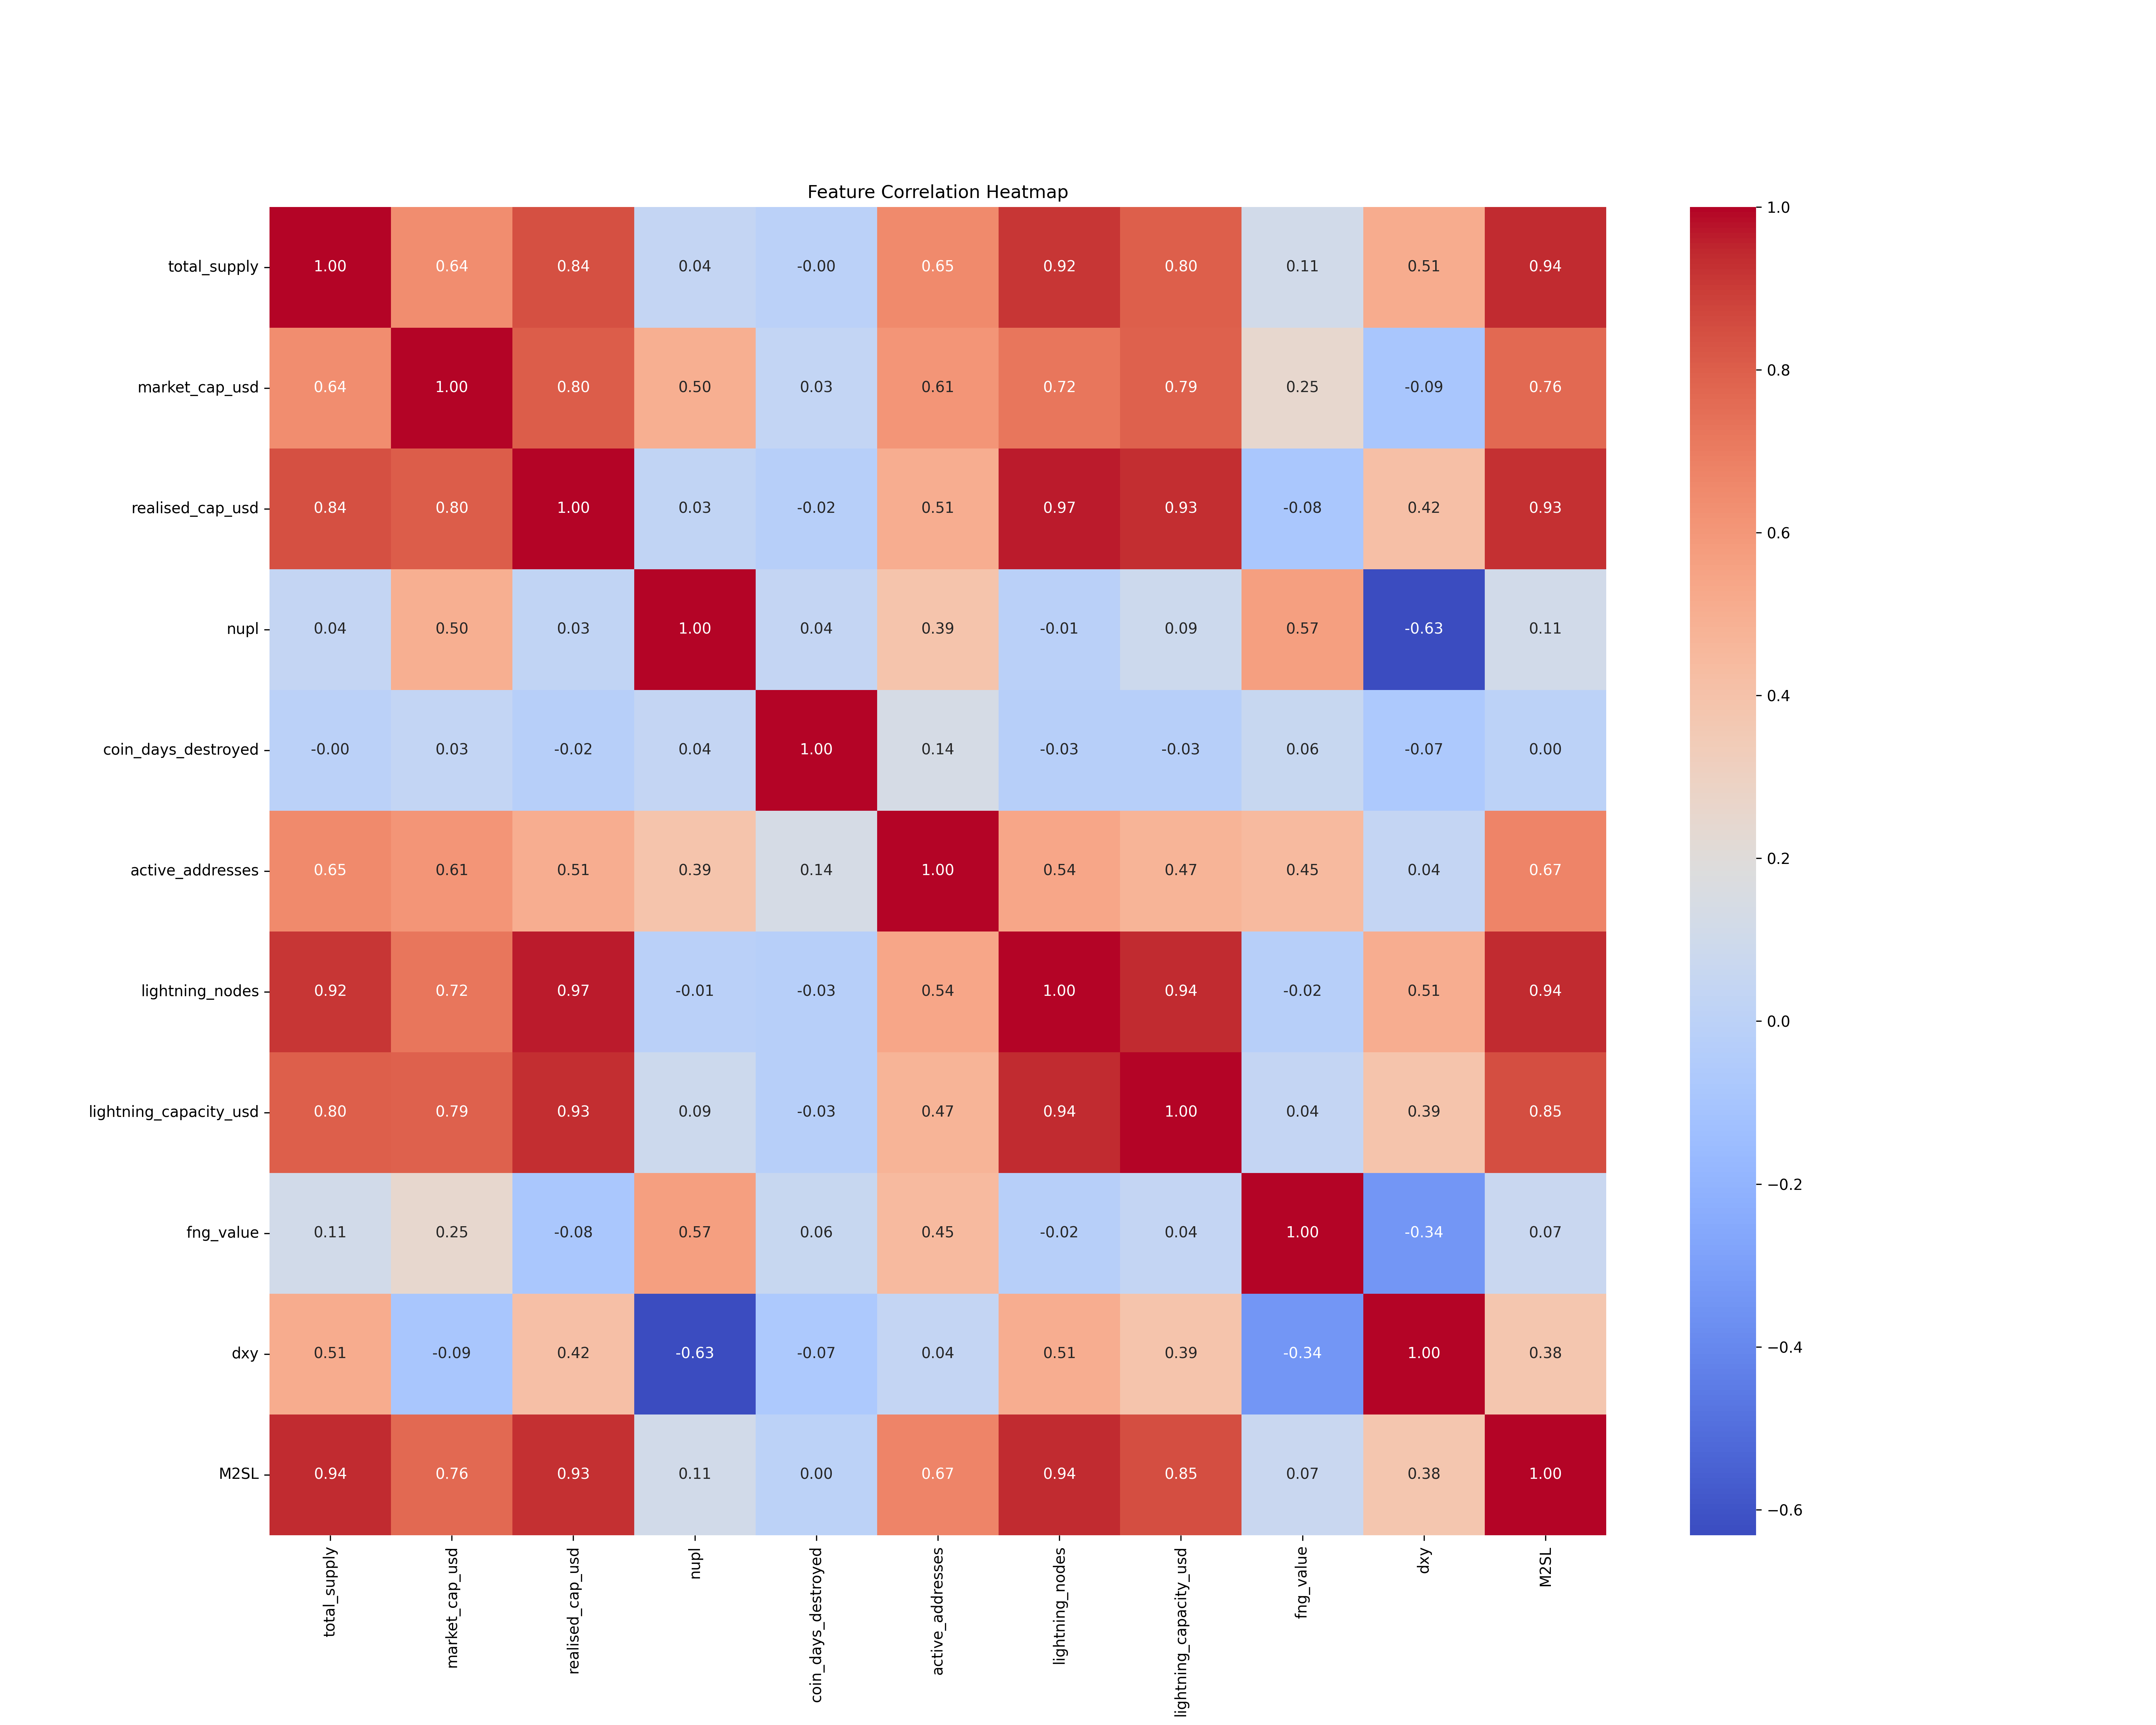
\includegraphics[width=0.5\textwidth]{plots/correlation_matrix_plot.png} % Replace with your file path
    \caption{Correlation Matrix.}
    \label{fig:correlation_matrix}
\end{figure}

Figure \ref{fig:correlation_matrix} shows the correlation matrix between various factors influencing the Bitcoin market.
The matrix visually represents how different variables such as Bitcoin price, M2SL, Fear and Greed index, and other
metrics are related to one another. High correlations suggest that certain factors move together, which can provide
important insights into the driving forces behind Bitcoin's price changes. The analysis of the correlation matrix is
key in identifying significant predictors for Bitcoin price forecasting.

This collection of figures together provides a comprehensive view of the factors influencing Bitcoin price movements,
sentiment, and economic context. Each figure serves as a piece of the puzzle in understanding how various macroeconomic
and market-specific variables interact and impact Bitcoin’s market performance.

\subsection{Data Preprocessing}\label{sec:data_preprocessing}

The data preprocessing process is a crucial step in preparing the raw dataset for further analysis and model training.
The preprocessing pipeline is implemented within the \texttt{DataPreprocessing} class, which performs several key
operations on the provided dataset.

The class initializes with a DataFrame (\texttt{data}) containing the raw dataset and two instances of
\texttt{StandardScaler} from the \texttt{sklearn} \texttt{.preprocessing} module, which are used for normalizing
the features and target variable.

\subsubsection{Loading and Saving Data}

To ensure smooth handling of data during the preprocessing, the class includes methods for saving and loading the
processed data. The \texttt{save} method writes the processed data to a Parquet file format, which offers efficient
storage. The \texttt{load} method reads in previously processed data from the same file format. The file is stored in
the \texttt{../data/processed\_data.parquet} directory.

\subsubsection{Data Transformation}

The core of the preprocessing happens in the \texttt{process} method, where the dataset undergoes several transformations:

\begin{enumerate}
    \item \textbf{Normalization of Dates:} The \texttt{date} column is first converted to represent the number of days'
                                           since the earliest date in the dataset. This is achieved by subtracting the
                                           minimum date (\texttt{reference\_date}) from each date in the \texttt{date}
                                           column and converting the result to days. This transformation makes it easier
                                           to handle the temporal aspect of the data in machine learning models, which
                                           typically perform better with numerical input rather than date objects.
    \item \textbf{Separation of Features and Target Variable:} The dataset is split into features (denoted as \texttt{x\_df})
                                                               and the target variable (denoted as \texttt{y\_df}). The target
                                                               variable in this case is \texttt{market\_price\_usd}, which
                                                               represents the price of Bitcoin, while all other columns become
                                                               the feature set.
    \item \textbf{Scaling of Features:} To ensure that all features are on a similar scale, which is critical for many machine
                                        learning algorithms, the features (\texttt{x\_df}) are standardized using the
                                        \texttt{StandardScaler}. This scales the data such that the mean is 0 and the standard
                                        deviation is 1. The scaled data is stored in \texttt{df\_x\_scaled}.
    \item \textbf{Scaling of Target Variable:} Similarly, the target variable (\texttt{y\_df}) is also scaled using a separate
                                               instance of \texttt{StandardScaler} to ensure that it is on the same scale as
                                               the features. The scaled target data is stored in \texttt{df\_y\_scaled}.
\end{enumerate}

Finally, the scaled feature and target datasets are saved as instance variables \texttt{df\_x\_scaled} and \texttt{df\_y\_scaled},
which can be used for further analysis or fed into machine learning models.

This preprocessing pipeline prepares the data by transforming it into a format suitable for statistical modeling and machine
learning, ensuring consistency and normalization across features and target variables.

\subsection{Model Tuning}\label{sec:model_tuning}

Model tuning is a critical step in optimizing machine learning models to achieve the best predictive performance.
This section details the tuning process applied to AdaBoost, Random Forest, and Support Vector Machine (SVM)
regressors. The tuning process involves hyperparameter optimization using cross-validation and grid search, with
model evaluation based on Mean Absolute Error (MAE), Mean Squared Error (MSE), and R-squared (R2) scores.

\subsubsection{Hyperparameter Tuning Strategy}

Each model undergoes hyperparameter tuning using a systematic search over a predefined parameter grid. The
models are evaluated using K-Fold cross-validation to ensure robustness and avoid overfitting. \\

\textbf{Cross-Validation Setup}

\begin{itemize}
    \item \textbf{K-Fold Splitting:} A 3-fold cross-validation (K=3) is used
    \item \textbf{Scoring Metrics:}
    \begin{itemize}
        \item \textbf{MAE:} Measures average absolute errors
        \item \textbf{MSE:} Penalizes larger errors more significantly
        \item \textbf{R2:} Measures goodness of fit
    \end{itemize}
    \item \textbf{Parallel Processing:} The n\_jobs parameter is set to self.nproc to utilize multiple CPU cores
\end{itemize}

\subsubsection{AdaBoost Regressor Tuning}\label{sec:adaboost_regressor_tuning}

AdaBoost tuning involves selecting the best combination of base estimator depth, learning rate, and number of
estimators. \\

\textbf{Hyperparameters:}

\begin{itemize}
    \item n\_estimators: [1, 200, 400, 600, 800]
    \item learning\_rate: [0.001, 0.005, 0.01, 0.05, 0.1, 0.5, 1.0]
    \item loss: [`linear', `square', `exponential']
\end{itemize}

\textbf{Optimization Process:}

\begin{itemize}
    \item A DecisionTreeRegressor is used as the base estimator with varying max\_depth values
    \item A GridSearchCV is conducted to find the best combination of hyperparameters
    \item The best model is selected based on the lowest MSE
\end{itemize}

\subsubsection{Random Forest Regressor Tuning}\label{sec:rf_regressor_tuning}

Random Forest tuning focuses on optimizing tree depth, number of estimators, feature
selection, and leaf node constraints. \\

\textbf{Hyperparameters:}

\begin{itemize}
    \item n\_estimators: [1, 100, 200, 300, ..., 900]
    \item max\_depth: [1, 3, 5]
    \item max\_features: [`linear', `square', `exponential']
    \item max\_leaf\_nodes: [2, 3, 5]
\end{itemize}

\textbf{Optimization Process:}

\begin{itemize}
    \item GridSearchCV is applied with K-Fold cross-validation
    \item The best model is selected based on MSE performance on test data
\end{itemize}

\subsubsection{Support Vector Machine Regressor Tuning}\label{sec:svm_regressor_tuning}

AdaBoost tuning involves selecting the best combination of base estimator depth, learning rate, and number of
estimators. \\

\textbf{Hyperparameters:}

\begin{itemize}
    \item C: [1, 200, 400, 600, 800]
    \item kernel: [0.001, 0.005, 0.01, 0.05, 0.1, 0.5, 1.0]
    \item gamma: [`linear', `square', `exponential']
\end{itemize}


\textbf{Optimization Process:}

\begin{itemize}
    \item GridSearchCV is performed across different kernel functions
    \item The best-performing model is selected based on the lowest MSE
\end{itemize}

\subsection{Model Evaluation and Selection}\label{sec:model_evaluation_and_selection}
Once the hyperparameter tuning is complete, the best models from each category are evaluated on
test data. The final step involves selecting the best model for deployment by comparing performance
metrics across all models. The tuned models are then combined into a weighted Voting Regressor,
where individual models are weighted based on their inverse MSE values.

Hyperparameter tuning significantly improves model performance by optimizing key parameters. The
AdaBoost, Random Forest, and SVM regressors undergo rigorous tuning and evaluation, ensuring that
the final model ensemble provides the best possible predictions.

The performance of the tuned model was assessed using key evaluation metrics. The results indicate
significant prediction errors, as reflected by the following values:

\begin{itemize}
    \item \textbf{Mean Absolute Error (MAE):} 34,028.35
    \item \textbf{Mean Squared Error (MSE):} 1,174,315,995.49
    \item \textbf{R² Score:} -4,491,936,135.06
\end{itemize}

These results suggest that the model struggles to accurately capture the underlying patterns in
the data. The high MAE and MSE values indicate substantial deviations between the predicted and
actual values, while the negative R² score suggests that the model performs worse than a simple
mean predictor. This highlights the need for further improvements, such as feature engineering,
alternative model architectures, or additional data preprocessing techniques to enhance prediction
accuracy.

From the results shown in Figure\ \ref{fig:prediction_vs_actual}, the model is able to somewhat 
predict the general price movement; however, struggles at predicting the large swings in Bitcoin's
price. The model may be underfitting the data too much resulting in highly inaccurat price predictions.

\begin{figure}[h]
    \centering
    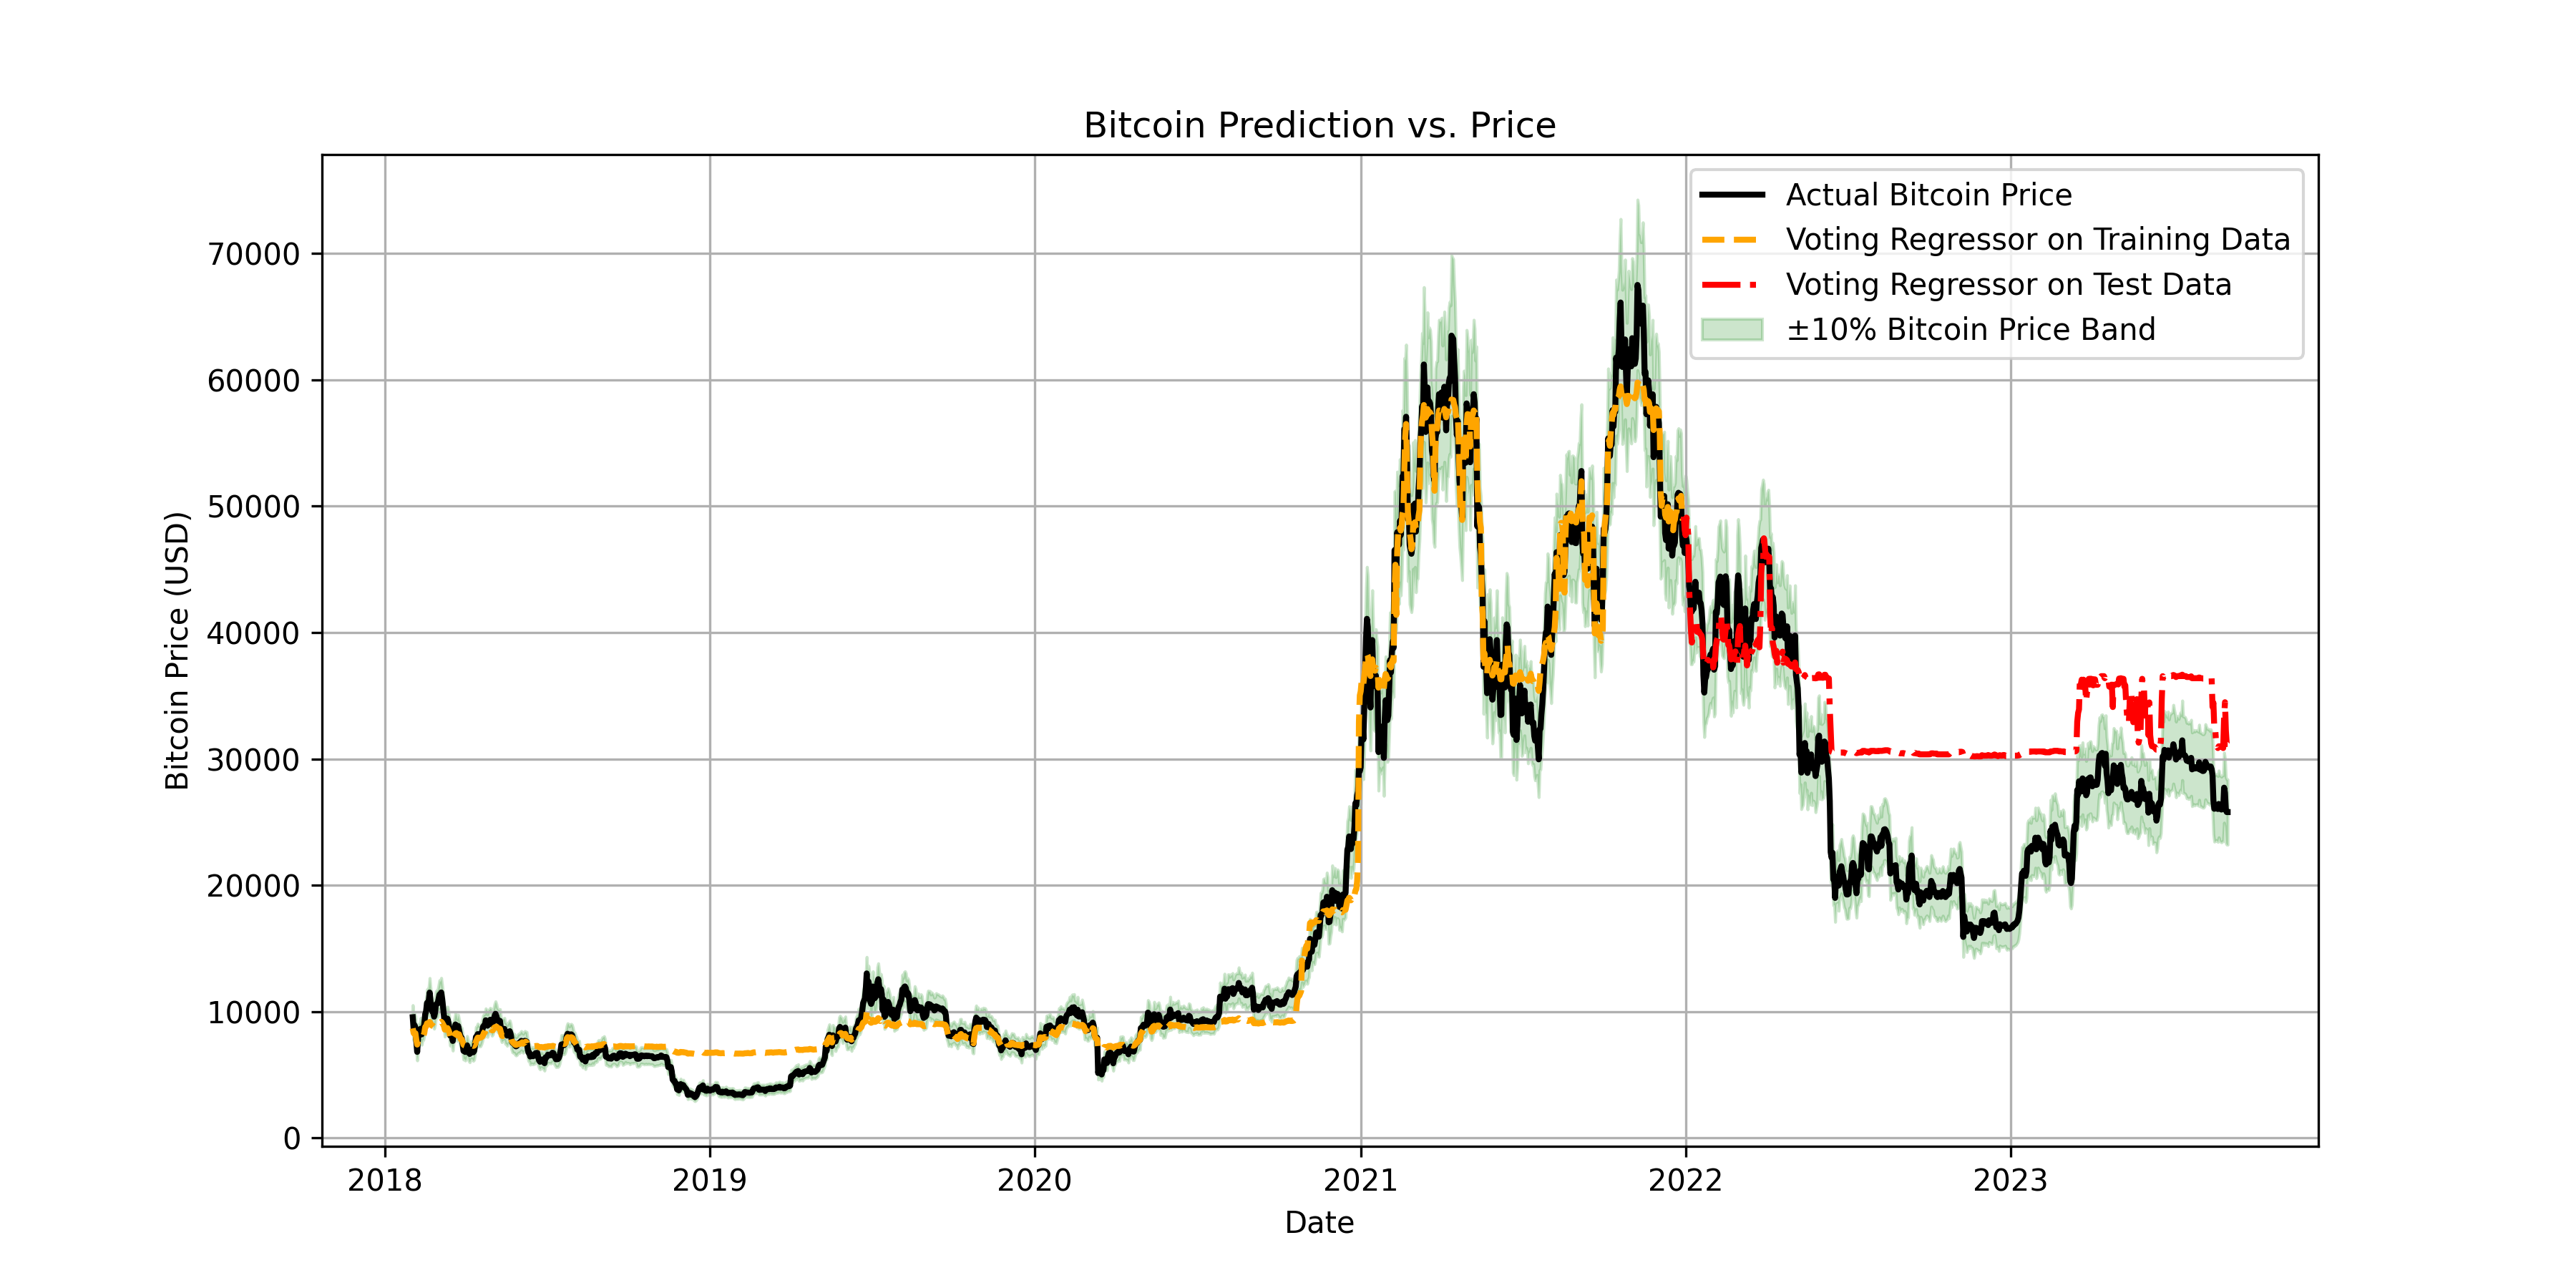
\includegraphics[width=0.5\textwidth]{plots/prediction_vs_actual.png} % Replace with your file path
    \caption{Bitcoin Price Data.}
    \label{fig:prediction_vs_actual}
\end{figure}



\section{Discussion}\label{sec:discussion}


\section{Conclusion}\label{sec:conclusion}

This work introduces a deep learning framework for spectral CT tissue decomposition, leveraging U-Net 
architectures to segment and quantify adipose, fibroglandular, and calcified tissues from dual-energy attenuation inputs. 
From utilizing the Beer–Lambert law, domain-specific feature construction, and deep convolutional 
networks, the method achieves high segmentation fidelity across tissue types, including rare calcification patterns.

Quantitative evaluation shows that the deeper \texttt{UNet512} model achieves the best performance, with a final validation 
loss of 0.0292 and mean absolute error below 0.003 for all tissue categories. Predicted tissue compositions closely match 
ground truth distributions, highlighting the model`s clinical relevance.

Overall, this study demonstrates that coupling physics-based domain knowledge with deep learning architectures offers a 
powerful and interpretable approach to spectral CT analysis. Future work will extend this model to real-world datasets, 
investigate 3D volumetric extensions, and incorporate uncertainty estimation to further enhance clinical utility.


\bibliographystyle{ACM-Reference-Format}
\bibliography{references.bib}

\end{document}
